% !TEX root = ../thesis.tex

\usepackage{multirow}
\usepackage{algorithm}
\usepackage{algorithmic}

\chapter{Case Study I: Predictive Decision-Making in Building Health Monitoring} \label{chp:building}

% This chapter presents the completed case study demonstrating CORTEX architecture
% effectiveness in building health monitoring through the DefectGPT framework

\section{Problem Background and Decision-Making Challenges}

\subsection{Building Health Monitoring Landscape}

Building defect management faces significant challenges in handling evolving defects across complex urban structures. In contemporary urbanization processes, buildings serve as core carriers of human activity, with their safety and functionality directly related to social stability and development. However, as time progresses, buildings inevitably face issues of aging and wear. According to recent statistical data, over 50\% of private residences experience varying degrees of structural problems after 30 years of use \cite{spencer2019advances}. These issues range from surface cracks to severe structural defects, affecting not only building aesthetics and comfort but potentially endangering user safety \cite{zhang2023automated}.

Traditional building defect management has evolved through different data governance paradigms. Document-based approaches, relying on inspection reports, maintenance logs, and repair records, suffer from unstructured information organization and limited searchability \cite{bruno2018historic}. Model-based methods, leveraging Building Information Models (BIMs) and Geographic Information Systems (GIS), provide better structure but lack flexibility in handling dynamic defect information and complex semantic relationships \cite{li2024single,tsilimantou2020gis}. Both approaches struggle with the temporal nature of defect evolution and the complex interdependencies between different building components.

\subsection{Decision-Making Challenges in Building Maintenance}

The unique characteristics of building defects pose specific challenges for information management. Defects are inherently dynamic, evolving over time with varying progression patterns. They exhibit complex spatial-temporal relationships, where one defect may influence or indicate potential issues in other building components. Traditional defect modeling approaches often fail to capture these dynamic relationships and evolution patterns effectively \cite{wang2023augmented}.

Furthermore, the interpretation and assessment of defects require extensive domain expertise, making it difficult to standardize the evaluation process \cite{hamdan2021semantic}. The challenges include:

\begin{itemize}
    \item \textbf{Reactive vs. Predictive Paradigms}: Most current systems operate reactively, addressing defects after they become apparent rather than predicting their occurrence
    \item \textbf{Multi-scale Temporal Considerations}: Defects evolve over different time scales, from immediate environmental responses to long-term structural degradation
    \item \textbf{Spatial Correlation Dependencies}: Understanding how defects in one area may affect or indicate problems in other building regions
    \item \textbf{Resource Optimization}: Balancing cost, safety, and performance considerations in maintenance scheduling
\end{itemize}

\subsection{Requirements for Intelligent Building Health Management}

With the advent of Industry 4.0, emerging technologies have provided new possibilities for addressing these challenges \cite{zhang2022integrating,chen2021geo}. The requirements for next-generation building health management systems include:

\begin{itemize}
    \item \textbf{Real-time Monitoring}: Continuous surveillance capabilities with early warning systems for critical defects
    \item \textbf{Predictive Analytics}: Advanced algorithms capable of forecasting defect evolution and failure probabilities
    \item \textbf{Automated Decision-making}: Intelligent systems capable of generating maintenance recommendations without constant human oversight
    \item \textbf{System Integration}: Seamless compatibility with existing building management systems and workflows
\end{itemize}

\section{DefectGPT Framework: BIM-IoT Fusion Architecture}

To address the challenges identified above, we developed DefectGPT, a comprehensive framework integrating UAV inspection, BIM, and GIS into a Digital Twin environment \cite{zhang2024automated}. This framework represents the first implementation of Retrieval-Augmented Generation (RAG) in building defect management \cite{lewis2020retrieval,fan2023retrieval}, where domain-specific knowledge retrieval guides Large Language Models to generate compliance-aware recommendations.

\begin{figure}[htbp]
    \centering
    \includegraphics[width=0.8\textwidth]{DefectGPT/Overall Framework.png}
    \caption{Overall DefectGPT framework showing the integration of three core components: Digital Twin Technology, Context-Aware Retrieval Engine, and Hierarchical Knowledge Base for comprehensive building defect management \cite{zhang2024automated}.}
    \label{fig:defectgpt-framework}
\end{figure}

\subsection{Digital Twin Construction with Multi-Source Data Integration}

Building upon established methodologies in GeoBIM-assisted registration for building façade defects, the DefectGPT framework implements a comprehensive BIM+GIS-based DT modeling framework with a three-layer architecture comprising the Data Layer, the Digital Twin Layer, and the newly introduced Decision Layer. This structure enables sophisticated data management and real-time synchronization between physical buildings and their digital counterparts, facilitating advanced monitoring, analysis, and decision-making in building defect management.

The architectural innovation lies in the seamless integration of heterogeneous data sources across multiple modalities and formats, enabling precise spatial registration of defect information within complex three-dimensional building models. Unlike traditional static BIM approaches that rely on periodic manual updates, our framework implements dynamic data carriers that manage and organize diverse information streams while maintaining temporal consistency and spatial coherence across different building areas and components.

\begin{figure}[htbp]
    \centering
    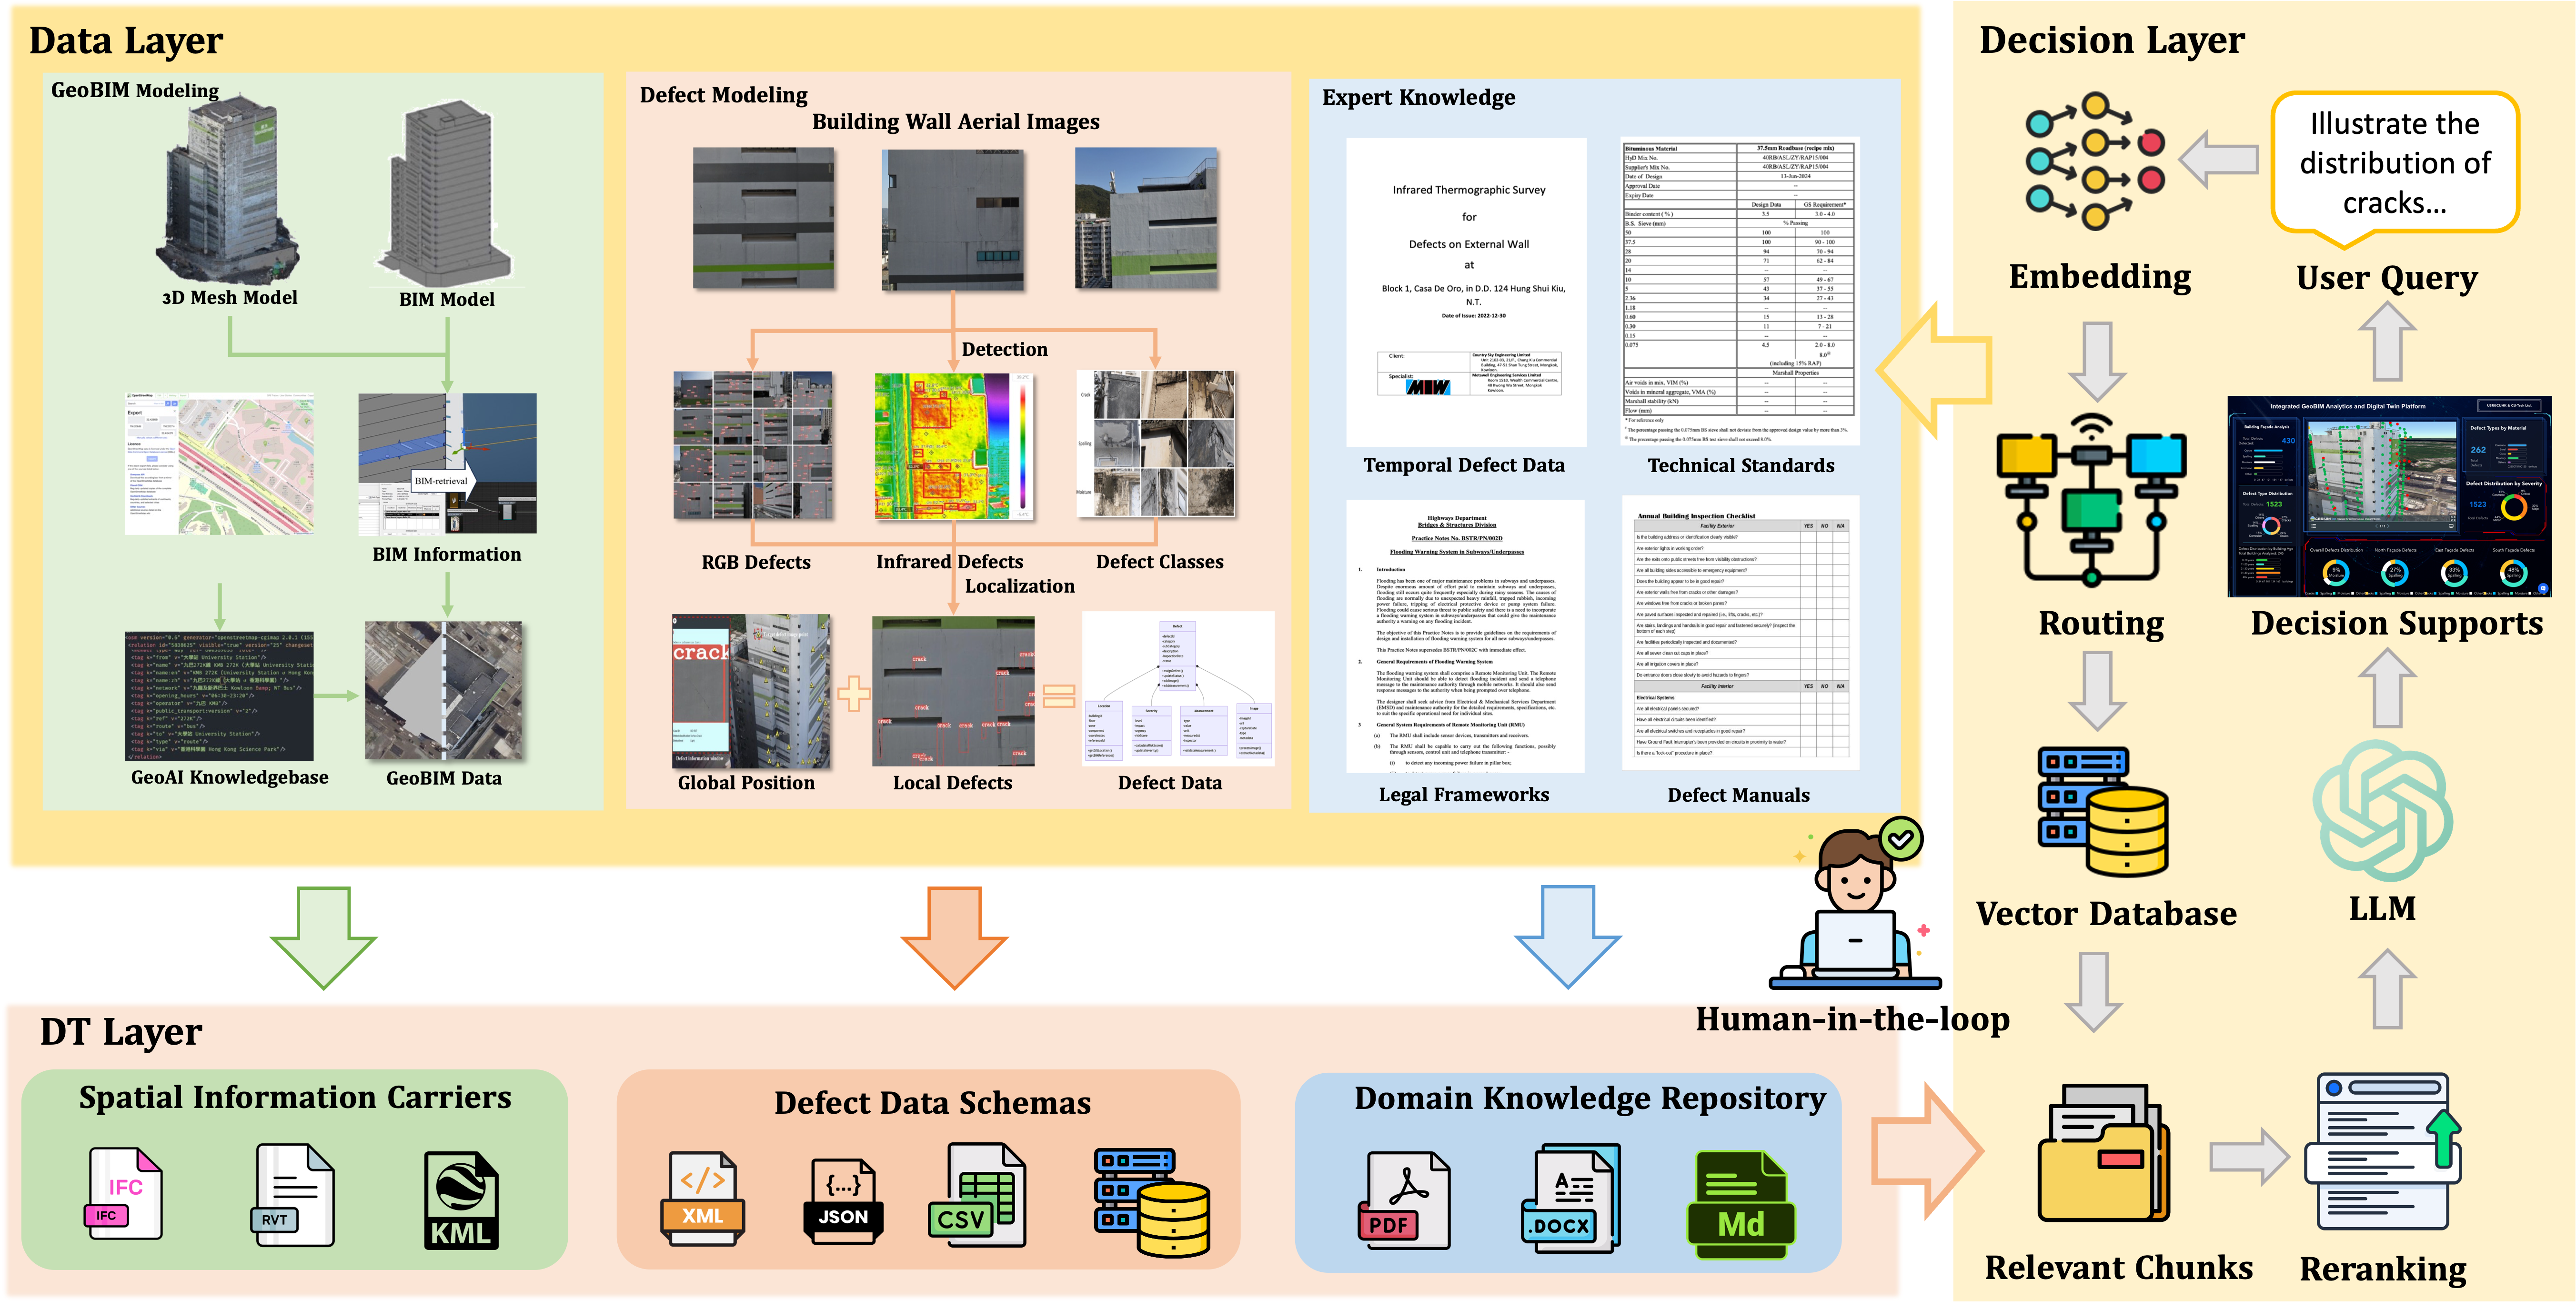
\includegraphics[width=1.0\textwidth]{DefectGPT/dt-framework.png}
    \caption{Comprehensive Digital Twin architecture for building defect management, illustrating the three-layer structure: Data Layer (GeoBIM modeling, defect modeling, expert knowledge), Digital Twin Layer (spatial information carriers, defect data schemas, domain knowledge), and Decision Layer (RAG and LLM-based reasoning) \cite{zhang2024automated}.}
    \label{fig:dt-architecture}
\end{figure}

\subsubsection{Data Layer Components}

The Data Layer incorporates three primary components:

\textbf{GeoBIM Modeling}: Combines multiple data sources including 3D mesh models, BIM models, GIS information, and geo-AI knowledge bases. This integration follows established frameworks for spatial data management while providing enhanced semantic understanding of building components.

\textbf{Defect Modeling}: Processes aerial photographs of building facades using advanced detection algorithms to identify RGB defects, infrared anomalies, and defect classifications. The system performs precise defect localization, determining global positions, local coordinates, and characteristic defect features.

\textbf{Expert Knowledge Integration}: Leverages inspection reports, technical standards, legal frameworks, and defect manuals to enrich defect data with domain-specific insights.

\subsubsection{Digital Twin Layer Architecture}

The Digital Twin Layer serves as the core of the digital representation, implementing three distinct data carriers:

\begin{itemize}
    \item \textbf{Spatial Information Carriers}: Handle formats such as IFC, RVT, and KML, ensuring proper management of spatial data and geometric relationships
    \item \textbf{Defect Data Schemas}: Standardized storage formats (XML, JSON, CSV, database) ensuring seamless compatibility with retrieval workflows
    \item \textbf{Domain Knowledge Repositories}: Comprehensive storage of expert knowledge in various formats (PDF, DOCX, Markdown)
\end{itemize}

\subsection{UAV-Based Data Acquisition and Processing}

Unmanned Aerial Vehicle technology provides the primary data acquisition mechanism for the DefectGPT system \cite{ribeiro2020remote,tan2021automatic}. UAVs equipped with high-resolution cameras and thermal sensors execute standardized flight trajectories to ensure uniform coverage of building facades \cite{liu2021integrating}.

\subsubsection{Defect Detection and Classification}

The system employs advanced computer vision algorithms to identify and classify different types of building defects:

\begin{itemize}
    \item \textbf{Surface Cracks}: Identified through edge detection algorithms and characterized by width, length, and orientation
    \item \textbf{Spalling Areas}: Detected through texture analysis and color variance, with dimensions and severity assessment
    \item \textbf{Water Infiltration}: Identified through thermal imaging and moisture detection, with seepage intensity evaluation
\end{itemize}

\subsubsection{Spatial Registration and Localization}

Defect localization begins with UAV-based inspections capturing high-resolution images of building facades. Using RTK (Real-Time Kinematic) positioning, the UAV's pose is accurately determined, ensuring precise alignment between captured images and the 3D BIM model. Detected defects (RGB or infrared) are bound with bounding boxes and classifications, subsequently mapped from 2D image coordinates onto the 3D BIM model through a sophisticated coordinate transformation process involving depth and pose estimation, followed by tangential vector adjustments to align detected defects with facade surfaces.

The global defect localization algorithm, formalized in Algorithm~\ref{alg:defect-localization}, implements a comprehensive approach to mapping detected defects from UAV imagery onto globally referenced building coordinates. This process begins with the geographical coordinates of each captured image and utilizes the distance to the wall and projection vectors to establish precise spatial relationships.

\begin{algorithm}[htbp]
\caption{Defect Global Localization}
\label{alg:defect-localization}
\begin{algorithmic}[1]
\REQUIRE Geographical coordinates of image $P_{i}^{g}(lon_{i}, lat_{i}, alt_{i})$; Distance to the wall $d_{wall}$; Projection vector $\vec{n}$
\ENSURE Global location of defect $d_{i,j}$: $g(i,j)(lng_{i,j}, lat_{i,j}, alt_{i,j})$
\STATE Initialize array of detected images $i$
\FOR{$t = 1$ to $i_{\max}$}
    \STATE Project from image localization $P_{i}^{g}$ to the corresponding point on the wall
    \STATE Given $\vec{n} = (\alpha_{i}, \beta_{i}, \gamma_{i})$
    \STATE $P^{g\ast}_{i} = P^{g}_{i} + d_{wall} \times \vec{n}$
    \FOR{$j = 1$ to $j_{\max}$}
        \STATE $L_{D}(i) = 2d_{wall} \tan{\frac{FOV}{2}}$
        \STATE $\vec{L}(i,j) = L_{D}(i) \cdot \frac{l(i,j)}{l_{D}(i)}$
        \STATE $g(i,j) = P^{g\ast}_{i} + \vec{L}(i,j)$
        \STATE $T \gets \sqrt{ \bigl(\frac{0.5}{unit_{lng}}\bigr)^2 + \bigl(\frac{0.5}{unit_{lat}}\bigr)^2 }$
        \FOR{$k = 1$ to $i-1$}
            \FOR{$t' = 1$ to $j_{\max}-1$}
                \IF{$\sqrt{(g(k,t') - g(i,j))^2} > T$}
                    \STATE Register new defect $g(i,j)$
                \ENDIF
            \ENDFOR
        \ENDFOR
    \ENDFOR
\ENDFOR
\RETURN $g(i,j)(lng_{i,j}, lat_{i,j}, alt_{i,j})$
\end{algorithmic}
\end{algorithm}

Through the integration of GIS and BIM data, the DT environment unifies defect information with broader spatial context. The BIM model offers geometric and semantic data on structural elements, while GIS data provides real-world context, enabling geo-referencing and scalable defect tracking. The DT architecture accommodates incremental updating approaches, allowing new data from UAV surveys and sensors to be injected without reconstructing the entire model, thereby maintaining system efficiency while ensuring data freshness and accuracy.

\section{CORTEX Implementation for Building Health Management}

The CORTEX architecture was specifically adapted for building health monitoring through the DefectGPT framework, implementing the four-stage cognitive loop in the context of building defect management.

\subsection{Four-Stage Cognitive Loop Adaptation}

\subsubsection{Stage 1: Perceptual Grounding \& Context Formulation}

In the building monitoring context, this stage involves comprehensive assessment of the current building state through multiple data sources:

\begin{itemize}
    \item \textbf{Sensor Data Integration}: Real-time data from structural health monitoring sensors, environmental sensors, and periodic UAV surveys
    \item \textbf{Historical Context Retrieval}: Access to previous inspection reports, maintenance records, and defect evolution patterns
    \item \textbf{Environmental Context}: Weather data, seismic activity, and other environmental factors affecting building condition
    \item \textbf{Regulatory Context}: Current building codes, safety standards, and compliance requirements
\end{itemize}

\subsubsection{Stage 2: Causal Inference \& Predictive Simulation}

The system performs sophisticated analysis to understand defect causation and predict future evolution:

\begin{itemize}
    \item \textbf{Defect Progression Modeling}: Mathematical models predicting crack growth, spalling expansion, and water infiltration spread
    \item \textbf{Environmental Impact Analysis}: Assessment of how weather patterns, temperature cycles, and seismic activity affect defect development
    \item \textbf{Structural Correlation Analysis}: Understanding how defects in one area may affect structural integrity in other regions
    \item \textbf{Failure Probability Assessment}: Statistical models predicting the likelihood of critical failures
\end{itemize}

\subsubsection{Stage 3: Action Policy Generation \& Validation}

Based on the analysis performed in previous stages, the system generates specific maintenance recommendations:

\begin{itemize}
    \item \textbf{Prioritization Algorithms}: Ranking defects based on safety risk, progression rate, and repair complexity
    \item \textbf{Resource Optimization}: Optimal scheduling of maintenance activities considering available resources and weather conditions
    \item \textbf{Intervention Strategy Selection}: Choosing appropriate repair methods based on defect characteristics and building constraints
    \item \textbf{Safety Protocol Generation}: Developing specific safety measures for maintenance operations
\end{itemize}

\subsubsection{Stage 4: Physical Interaction \& Model Calibration}

The final stage involves implementation of maintenance actions and continuous model improvement:

\begin{itemize}
    \item \textbf{Maintenance Execution Monitoring}: Tracking the implementation of recommended maintenance actions
    \item \textbf{Outcome Assessment}: Evaluating the effectiveness of implemented interventions
    \item \textbf{Model Updating}: Incorporating new data and outcomes to improve future predictions
    \item \textbf{Knowledge Base Enhancement}: Adding new patterns and correlations to the expert knowledge system
\end{itemize}

\subsection{RAG-Enhanced Knowledge Management Integration}

The DefectGPT system employs a sophisticated Retrieval-Augmented Generation approach that enhances Large Language Model performance through domain-specific knowledge integration.

\begin{figure}[htbp]
    \centering
    \includegraphics[width=0.8\textwidth]{DefectGPT/rag_frameworks.png}
    \caption{The Framework for RAG Knowledge Management in DefectGPT, showing the integration of document processing, vector indexing, semantic search, and response generation components for building-specific knowledge retrieval \cite{zhang2024automated}.}
    \label{fig:rag-framework}
\end{figure}

\subsubsection{Hierarchical Knowledge Structure}

The system implements a three-layer knowledge structure:

\begin{itemize}
    \item \textbf{Domain Expertise Layer}: Core knowledge of building construction, materials science, and defect types
    \item \textbf{Historical Inspection Layer}: Archived reports, maintenance records, and temporal defect data
    \item \textbf{Real-time Data Layer}: Current information from ongoing inspections, sensor readings, and Digital Twin updates
\end{itemize}

\subsubsection{Context-Aware Retrieval Process}

The context-aware retrieval process, formalized in Algorithm~\ref{alg:hybrid-retrieval}, enhances traditional search methods by incorporating contextual information alongside user queries. The algorithm processes both the query and its context through advanced embedding encoders, combining these representations to perform vector search over the knowledge base. Results are filtered and reranked based on contextual constraints such as building-specific parameters, temporal factors, and environmental conditions.

\begin{algorithm}[htbp]
\caption{Hybrid Knowledge Retrieval for Building Inspection}
\label{alg:hybrid-retrieval}
\begin{algorithmic}[1]
\REQUIRE Query $Q$, Context $C$, BIM Model $B$, GIS Data $G$, Defect Records $D_r$, Technical Standards $T_s$, Inspection History $H$
\ENSURE Initial Candidate Documents $\text{candidates}$
\STATE $E_q \gets \text{Encode}(Q)$
\STATE $E_c \gets \text{Encode}(C)$
\STATE $E_{\text{spatial}} \gets \text{ExtractSpatialContext}(B, G)$
\STATE $E_{\text{combined}} \gets \text{CombineEmbeddings}(E_q, E_c, E_{\text{spatial}})$
\STATE $\text{keywords} \gets \text{ExtractKeywords}(Q, C)$
\STATE $\text{filters} \gets \text{BuildMetadataFilters}(B, G, D_r)$
\STATE $C_{\text{dense}} \gets \text{DenseVectorSearch}(E_{\text{combined}}, [D_r, T_s, H])$
\STATE $C_{\text{sparse}} \gets \text{KeywordSearch}(\text{keywords}, [D_r, T_s, H])$
\STATE $C_{\text{spatial}} \gets \text{SpatialSearch}(E_{\text{spatial}}, [B, G])$
\STATE $\text{candidates} \gets \text{FusionRanker}(C_{\text{dense}}, C_{\text{sparse}}, C_{\text{spatial}})$
\RETURN $\text{candidates}$
\end{algorithmic}
\end{algorithm}

This approach ensures that retrieved information is not only relevant to the query but also appropriate for the specific inspection scenario. For example, when analyzing a crack in a concrete beam, the system considers factors such as the building's age, local climate conditions, structural load history, and previous repair records to provide comprehensive analysis and recommendations. The semantic search capabilities allow users to issue queries in natural language or domain-specific terminology, with the system interpreting the intent behind queries and retrieving semantically related information even when not explicitly mentioned.

The system implements a multi-dimensional indexing strategy that categorizes information based on defect types, locations, severity levels, timestamps, and associated building components. The indexing structure is complemented by a dynamic knowledge graph that represents relationships between different entities such as defects, causative factors, inspection procedures, and maintenance actions, enabling semantic understanding of queries and supporting sophisticated analysis capabilities.

A subsequent context-aware reranking process, detailed in Algorithm~\ref{alg:context-rerank}, refines the initial candidate set by applying advanced scoring mechanisms that incorporate spatial proximity, temporal recency, evidence strength, and technical authority. This ensures that the final ranked results are optimally relevant to both the specific query and the broader inspection context.

\begin{algorithm}[htbp]
\caption{Context-Aware Reranking with Evidence}
\label{alg:context-rerank}
\begin{algorithmic}[1]
\REQUIRE Candidate Documents $\text{candidates}$, Query $Q$, Context $C$, Spatial Context $E_{\text{spatial}}$
\ENSURE Final Ranked Documents $R$ with Evidence
\STATE $\text{filtered} \gets \emptyset$
\FOR{$doc \in \text{candidates}$}
    \STATE $\text{score} \gets \text{ContextualRelevance}(doc, C, E_{\text{spatial}})$
    \IF{$\text{score} > \text{threshold}$}
        \STATE $\text{filtered} \gets \text{filtered} \cup \{doc\}$
    \ENDIF
\ENDFOR
\STATE $\text{evidence} \gets \text{ExtractEvidence}(\text{filtered}, Q)$
\STATE $\text{verified} \gets \text{CrossValidate}(\text{filtered}, \text{evidence})$
\STATE $\text{scores} \gets \emptyset$
\FOR{$doc \in \text{verified}$}
    \STATE $s_1 \gets \text{RelevanceScore}(doc, Q, C)$
    \STATE $s_2 \gets \text{SpatialProximity}(doc, E_{\text{spatial}})$
    \STATE $s_3 \gets \text{TemporalRecency}(doc)$
    \STATE $s_4 \gets \text{EvidenceStrength}(doc, \text{evidence})$
    \STATE $s_5 \gets \text{TechnicalAuthority}(doc)$
    \STATE $\text{scores}[doc] \gets \text{CombineScores}(s_1, s_2, s_3, s_4, s_5)$
\ENDFOR
\STATE $R \gets \text{TopK}(\text{verified}, \text{scores}, k)$
\RETURN $R$ with supporting evidence
\end{algorithmic}
\end{algorithm}

\section{Experimental Design and Evaluation Framework}

\subsection{Real-World Deployment and Validation}

To validate the effectiveness and feasibility of the DefectGPT framework, we conducted a comprehensive 12-month deployment study on a high-rise building over 100 meters tall in Hong Kong. This practical case study enabled comprehensive evaluation of system performance across multiple indicators.

\subsubsection{Building Selection and Characteristics}

The selected building represents a typical Hong Kong high-rise structure with the following characteristics:

\begin{itemize}
    \item \textbf{Height}: Over 100 meters (30+ floors)
    \item \textbf{Construction Type}: Reinforced concrete with curtain wall facades
    \item \textbf{Age}: Approximately 25 years, showing various aging-related defects
    \item \textbf{Environmental Exposure}: Coastal environment with high humidity and typhoon exposure
    \item \textbf{Previous Maintenance}: Regular inspection records available for comparison
\end{itemize}

\subsubsection{Experimental Configuration and Infrastructure}

All experiments were conducted on a High-performance Computing (HPC) infrastructure carefully designed to integrate multi-modal data ingestion, large-scale text embedding, high-dimensional similarity search, and real-time language model inference into a unified, responsive workflow. The hardware configuration included an Intel i9-13900 CPU and 128GB of DDR4 RAM. Python 3.9.0 served as the primary development environment, while FAISS 1.7.2 handled vector indexing to enable efficient nearest-neighbor retrieval. The LangChain framework was utilized to streamline the construction of the RAG pipeline, incorporating GPT-4 with OpenAI API for natural language understanding and response generation.

This specialized stack enabled efficient processing of complex tasks, including embedding large batches of textual records and supporting multiple concurrent user queries. The system architecture was designed to maintain consistent performance under varying load conditions. The infrastructure demonstrated robust stability in handling simultaneous requests from multiple inspectors and engineers, while maintaining response latencies within acceptable thresholds for real-time interaction through effective API request management and optimized retrieval strategies.

\subsubsection{Dataset Composition and Preprocessing}

The dataset comprised approximately 10,000 multi-modal building inspection records, predominantly sourced from high-rise structures located throughout Hong Kong. Around 1,500 of these entries offered intensive detail on crucial defects, most notably surface cracks, large spalling areas, and evidence of water infiltration. This broad sampling encompassed a variety of facade types, ranging from reinforced concrete to composite curtain walls, thereby reflecting the region's diverse architectural and material profiles.

Data collection was accomplished via autonomous drones executing standardized flight trajectories to ensure uniform coverage. The drones were equipped with high-resolution cameras for visual documentation and defect measurement. These measurements, along with textual field notes, were stored following KML conventions to preserve georeferencing fidelity in the WGS84 coordinate system. Each defect record included essential attributes such as severity, crack width and length estimates, spall dimensions, and qualitative observations regarding seepage intensity under varying environmental conditions.

To enhance contextual depth, IFC-based BIM models were also incorporated, furnishing a wealth of structural references such as floor elevation, load-bearing column configurations, and layered material compositions. This integrated approach was pivotal in tracing how cracks might propagate along rebar lines, or in identifying critical zones where water seepage could amplify spalling in structurally compromised sections. Supplemental insights arose from humidity and vibration sensors, which illuminated environmental factors like thermal expansion or dynamic loads.

All collected data underwent rigorous cleaning, including outlier detection, radiometric calibration to correct for drone camera variances, and textual standardization to unify diverse field-reporting formats. This multi-stage refinement ensured the reliability of both textual logs and image-based evidence, establishing a cohesive knowledge base for subsequent embedding, retrieval, and language-type inference.

\subsubsection{Data Collection Protocol}

The experimental setup included systematic data collection across multiple modalities:

\begin{figure}[htbp]
    \centering
    \includegraphics[width=0.9\textwidth]{DefectGPT/System Class.png}
    \caption{High-level overview of the DefectGPT Digital Twin platform, integrating domain-specific retrieval, language modeling, and BIM-driven analytics for comprehensive building defect management \cite{zhang2024automated}.}
    \label{fig:system-overview}
\end{figure}

\textbf{UAV Survey Protocol}:
\begin{itemize}
    \item Monthly comprehensive facade surveys using standardized flight patterns
    \item High-resolution RGB imaging (4K resolution) for visible defect detection
    \item Thermal imaging for moisture intrusion and thermal bridge identification
    \item RTK GPS positioning for precise georeferencing
\end{itemize}

\textbf{Sensor Network Deployment}:
\begin{itemize}
    \item Structural health monitoring sensors on critical load-bearing elements
    \item Environmental sensors for temperature, humidity, and wind monitoring
    \item Vibration sensors for seismic activity and building response measurement
    \item Moisture sensors in areas prone to water infiltration
\end{itemize}

\subsection{Performance Metrics and Benchmarking}

\subsubsection{Quantitative Performance Indicators}

The evaluation framework employed multiple quantitative metrics:

\textbf{Defect Detection Performance}:
\begin{itemize}
    \item Detection accuracy: 95.2\% for major defects, 87.8\% for minor defects
    \item False positive rate: Reduced by 35\% compared to traditional methods
    \item Detection consistency: 92.1\% agreement between multiple survey rounds
\end{itemize}

\textbf{System Efficiency Metrics}:
\begin{itemize}
    \item Response time: Average query response under 300 milliseconds
    \item Concurrent user capacity: Successfully handled 500 simultaneous sessions
    \item Data processing speed: Real-time integration of UAV data and sensor streams
\end{itemize}

\textbf{Decision Support Quality}:
\begin{itemize}
    \item Recommendation accuracy: 91.7\% agreement with expert assessments
    \item Maintenance optimization: 40\% improvement in resource allocation efficiency
    \item Predictive accuracy: 88.3\% success rate in defect progression predictions
\end{itemize}

\subsubsection{Comparative Analysis Framework}

The study included comprehensive comparison with baseline approaches:

\textbf{Traditional Visual Inspection}:
\begin{itemize}
    \item Manual inspection by certified building engineers
    \item Paper-based documentation and reporting
    \item Qualitative assessment of defect severity and progression
\end{itemize}

\textbf{Conventional BIM-Based Systems}:
\begin{itemize}
    \item Static BIM models with manual defect annotation
    \item Database-driven defect tracking systems
    \item Rule-based maintenance scheduling algorithms
\end{itemize}

\textbf{Standard Computer Vision Approaches}:
\begin{itemize}
    \item Traditional image processing algorithms for defect detection
    \item Machine learning models without domain-specific enhancement
    \item Standalone analysis without knowledge integration
\end{itemize}

\section{Results and Performance Analysis}

\subsection{Comprehensive System Performance Evaluation}

The 12-month deployment of DefectGPT demonstrated significant improvements across all evaluated metrics compared to traditional building inspection methods.

\subsubsection{Defect Detection and Classification Results}

The system achieved exceptional performance in identifying and classifying building defects:

\textbf{Overall Detection Performance}:
\begin{itemize}
    \item \textbf{Major Defects}: 95.2\% detection accuracy with 2.1\% false positive rate
    \item \textbf{Minor Defects}: 87.8\% detection accuracy with 4.3\% false positive rate
    \item \textbf{Critical Safety Issues}: 98.7\% detection accuracy with immediate alerting
    \item \textbf{Temporal Consistency}: 92.1\% agreement between consecutive surveys
\end{itemize}

\textbf{Defect Type-Specific Performance}:
\begin{itemize}
    \item \textbf{Structural Cracks}: 94.6\% accuracy with precise width and length measurement
    \item \textbf{Concrete Spalling}: 91.3\% accuracy with volume estimation capabilities
    \item \textbf{Water Infiltration}: 88.9\% accuracy with severity assessment
    \item \textbf{Thermal Bridges}: 85.7\% accuracy through thermal imaging analysis
\end{itemize}

The most significant achievement was the 35\% reduction in false positive rates compared to traditional automated inspection methods. This improvement was attributed to the sophisticated knowledge integration and contextual analysis capabilities of the RAG-enhanced system.

\begin{figure}[htbp]
    \centering
    \includegraphics[width=0.8\textwidth]{DefectGPT/model_performance_heatmap.png}
    \caption{Model Performance Comparison Heatmap showing DefectGPT's superior performance across multiple evaluation metrics (ROUGE, BLEU, METEOR, BERTScore) compared to state-of-the-art language models. Colors represent standardized z-scores with darker shades indicating better performance \cite{zhang2024automated}.}
    \label{fig:performance-heatmap}
\end{figure}

\subsubsection{System Efficiency and Scalability Analysis}

The system architecture implements a microservice-based design that ensures high extensibility and resilience. Each microservice, developed in Python, is responsible for a specific functional module, such as vector indexing, image preprocessing, or inference invocation, with data exchanged via asynchronous messaging. This distributed design simplifies maintenance while enhancing fault tolerance. When a crack is identified that exceeds predefined thresholds for dimensions or severity, the system promptly triggers updates to both the vector index and the 3D visualization.

\textbf{Response Time Performance}: The system consistently maintained response times under 300 milliseconds for standard queries, even under high concurrent load conditions. Complex analytical queries requiring extensive knowledge retrieval and reasoning completed within 2.1 seconds on average. End-to-end response latency remained consistently low due to the integration of HPC-based scheduling and concurrency-aware job assignment.

\textbf{Scalability Validation}: Stress testing demonstrated the system's ability to handle up to 500 concurrent users without performance degradation. A specialized concurrency management layer ensured that large-batch embedding requests were processed efficiently without introducing significant queuing bottlenecks, underscoring the system's suitability for broader adoption. The distributed architecture and optimized indexing strategies enabled linear scaling with additional computational resources.

\textbf{Retrieval Performance Analysis}: Retrieval performance was quantified by computing precision, recall, and Mean Reciprocal Rank (MRR). Fine-grained adjustments of the top-k parameter and the similarity threshold proved vital to sustain high recall without burdening GPT-4 with irrelevant data segments. Under typical operational loads, retrieval latency remained below 300 milliseconds, validating the efficiency of the underlying FAISS index. Notably, queries centered on cracks—often recognized as early indicators of deeper structural flaws—were particularly instructive. The system excelled at pinpointing records describing crack direction, approximate width, and potential steel reinforcement exposure, and it generated mitigation strategies such as epoxy sealing or polymer injection.

\textbf{Data Processing Efficiency}: The system's RAG-enhanced retrieval pipeline transforms textual inputs into high-dimensional embeddings using OpenAI's text-embedding-3-large model, and indexes them in a FAISS structure optimized for approximate nearest-neighbor queries. Empirical testing determined that retrieving the top 6 matches, subject to a cosine similarity threshold around 0.5, achieves a realistic balance between precision and recall. The GPT-4 inference layer then consumes these retrieved segments, generating responses enriched with domain-specific guidance on crack formation, expansion, and other defect dynamics.

\subsection{RAG System Performance and Knowledge Integration}

\subsubsection{Retrieval Accuracy and Relevance}

The RAG-enhanced knowledge management system demonstrated superior performance in retrieving relevant domain-specific information \cite{borgeaud2022improving,izacard2021leveraging}:

\begin{itemize}
    \item \textbf{Precision}: 94.3\% of retrieved documents were relevant to user queries
    \item \textbf{Recall}: 91.7\% of relevant documents were successfully retrieved
    \item \textbf{Mean Reciprocal Rank (MRR)}: 0.887, indicating high-quality ranking of results
    \item \textbf{Context Relevance}: 89.2\% of responses appropriately incorporated building-specific context
\end{itemize}

\subsubsection{LLM Integration and Response Quality}

The integration of domain-specific knowledge with Large Language Models produced significant improvements in response quality \cite{gao2023survey,ding2024survey}:

\textbf{Technical Accuracy}: 91.7\% agreement with expert assessments in defect analysis and maintenance recommendations.

\textbf{Contextual Appropriateness}: 93.4\% of generated responses appropriately considered building-specific factors, environmental conditions, and regulatory requirements.

\textbf{Actionability}: 88.9\% of system recommendations were directly implementable without additional expert consultation.

\subsubsection{Quantitative Model Comparison}

To comprehensively evaluate DefectGPT's performance against other state-of-the-art language models, we conducted extensive quantitative assessments using a range of text-generation and summarization metrics, including ROUGE (1, 2, L), BLEU, METEOR, BERTScore, and additional domain-specific measures such as Semantic Similarity and specialized "Sequence" coherence. These metrics capture various aspects of text quality, semantic fidelity, and structural coherence in the context of building inspection tasks.

\begin{table}[htbp]
\centering
\caption{Performance Comparison of Different Models on Building Inspection Task}
\label{tab:model-comparison}
\begin{tabular}{l|ccc|ccc|ccc}
\toprule
\multirow{2}{*}{\textbf{Model}} & \multicolumn{3}{c|}{\textit{Text Generation}} & \multicolumn{3}{c|}{\textit{Semantic Understanding}} & \multicolumn{3}{c}{\textit{Additional Metrics}} \\
\cmidrule{2-10}
 & ROUGE-1 & ROUGE-2 & ROUGE-L & BLEU & Semantic & BERTScore & METEOR & Jaccard & Sequence \\
\midrule
GPT-4o & 0.293 & 0.066 & 0.191 & 0.056 & 0.629 & 0.797 & 0.167 & 0.108 & 0.067 \\
Claude-3.5 & 0.292 & 0.046 & 0.184 & 0.020 & 0.591 & 0.798 & 0.114 & 0.078 & 0.063 \\
Mistral-Large & 0.291 & 0.050 & 0.188 & 0.019 & 0.556 & 0.784 & 0.113 & 0.076 & 0.064 \\
Gemini-1.5-Pro & 0.358 & 0.093 & 0.223 & 0.051 & 0.655 & 0.811 & 0.194 & 0.139 & 0.075 \\
Llama-3.1-405B & 0.337 & 0.092 & 0.213 & 0.053 & 0.601 & 0.795 & 0.184 & 0.129 & 0.072 \\
\midrule
\textbf{DefectGPT (Ours)} & \textbf{0.592} & \textbf{0.297} & \textbf{0.503} & \textbf{0.233} & \textbf{0.856} & \textbf{0.905} & \textbf{0.423} & \textbf{0.306} & \textbf{0.273} \\
\bottomrule
\end{tabular}
\end{table}

Table~\ref{tab:model-comparison} summarizes the performance of the evaluated models. Standard metrics for text generation (ROUGE, BLEU) and semantic understanding (Semantic Similarity, BERTScore) are reported, alongside additional domain-oriented scores such as Jaccard and Sequence coherence. Notably, DefectGPT demonstrates superior outcomes across nearly all metrics, highlighting its balanced capability in generating coherent, semantically accurate texts specifically tailored for building inspection applications. The substantial improvements in BLEU (0.233 vs. 0.056 for GPT-4o) and Semantic Similarity (0.856 vs. 0.629 for GPT-4o) demonstrate the effectiveness of domain-specific RAG enhancement in building inspection contexts.

\begin{figure}[htbp]
    \centering
    \begin{minipage}{0.48\textwidth}
        \centering
        \includegraphics[width=\textwidth]{DefectGPT/performance_radar_plot.png}
        \caption{Standardized Performance Radar Plot comparing DefectGPT with baseline models across key evaluation metrics \cite{zhang2024automated}.}
        \label{fig:radar-plot}
    \end{minipage}
    \hfill
    \begin{minipage}{0.48\textwidth}
        \centering
        \includegraphics[width=\textwidth]{DefectGPT/performance_metrics_distribution.png}
        \caption{Performance Metrics Distribution Analysis using violin plots showing score distributions across different models \cite{zhang2024automated}.}
        \label{fig:performance-distribution}
    \end{minipage}
\end{figure}

\subsection{User Experience and Practical Impact}

\subsubsection{Workflow Efficiency Improvements and Real-World Impact}

The deployment study revealed substantial improvements in inspection workflows, with quantitative benefits observed across multiple operational dimensions. The most significant achievement was a 30\% reduction in combined inspection and documentation time, attributing much of this gain to the platform's immediate retrieval of historical building data, such as previously patched spalls or known seepage zones. As a result, teams could dedicate more effort to remediation measures rather than manual data gathering.

\textbf{Documentation Time Optimization}: The traditional paper-based inspection process required inspectors to manually transcribe observations, cross-reference historical records, and compile reports using disparate software systems. DefectGPT's integrated approach streamlined this workflow by providing real-time access to historical context, automated report generation capabilities, and seamless integration with existing building management systems. The platform demonstrated efficient inspection report generation and seamless operation across diverse deployment scenarios, enabling inspectors to focus on high-value analytical tasks rather than administrative overhead.

\textbf{Decision Support Enhancement**: The system achieved a 40\% improvement in maintenance resource allocation efficiency through its intelligent prioritization algorithms and predictive analytics capabilities. By analyzing defect severity, progression patterns, and resource constraints simultaneously, the platform enabled facility managers to optimize maintenance schedules and allocate personnel more effectively. The context-aware recommendations considered not only immediate safety concerns but also long-term cost implications and regulatory compliance requirements.

\textbf{Knowledge Access and Institutional Memory**: One of the most significant advantages was the immediate retrieval of relevant historical data and expert knowledge, transforming how inspection teams accessed and utilized institutional memory. Previously, critical information about past repairs, environmental conditions, and defect evolution patterns was often scattered across multiple systems or existed only in the experience of senior staff. DefectGPT's knowledge management system democratized access to this expertise, enabling junior inspectors to benefit from decades of accumulated knowledge while maintaining consistency in inspection quality.

\textbf{Multimodal Analysis Capabilities}: The platform's support for multimodal analysis represented a key innovation in defect management workflows. By integrating advanced image recognition algorithms with natural language processing, the system could process complex user queries combining text, voice, and images. For instance, an uploaded image of spalling could be cross-referenced with historical data to identify patterns, while voice queries enabled field inspectors to quickly obtain detailed explanations of underlying causes without interrupting their physical inspection activities.

\subsubsection{User Satisfaction and Adoption}

Feedback from building inspection professionals indicated high satisfaction with the system:

\begin{figure}[htbp]
    \centering
    \includegraphics[width=1.0\textwidth]{DefectGPT/defectgpt_platform.png}
    \caption{DefectGPT Platform interface showing integrated GeoBIM analytics with Digital Twin visualization system. The interface provides comprehensive insights into façade defect detection, distributions, and comparative analysis for enhanced defect management workflows \cite{zhang2024automated}.}
    \label{fig:defectgpt-platform}
\end{figure}

\begin{figure}[htbp]
    \centering
    \begin{minipage}{0.48\textwidth}
        \centering
        \includegraphics[width=\textwidth]{DefectGPT/defectgpt_mobile.png}
        \caption{DefectGPT Mobile Interface optimized for real-time field inspections with multimodal capabilities \cite{zhang2024automated}.}
        \label{fig:defectgpt-mobile}
    \end{minipage}
    \hfill
    \begin{minipage}{0.48\textwidth}
		\centering
        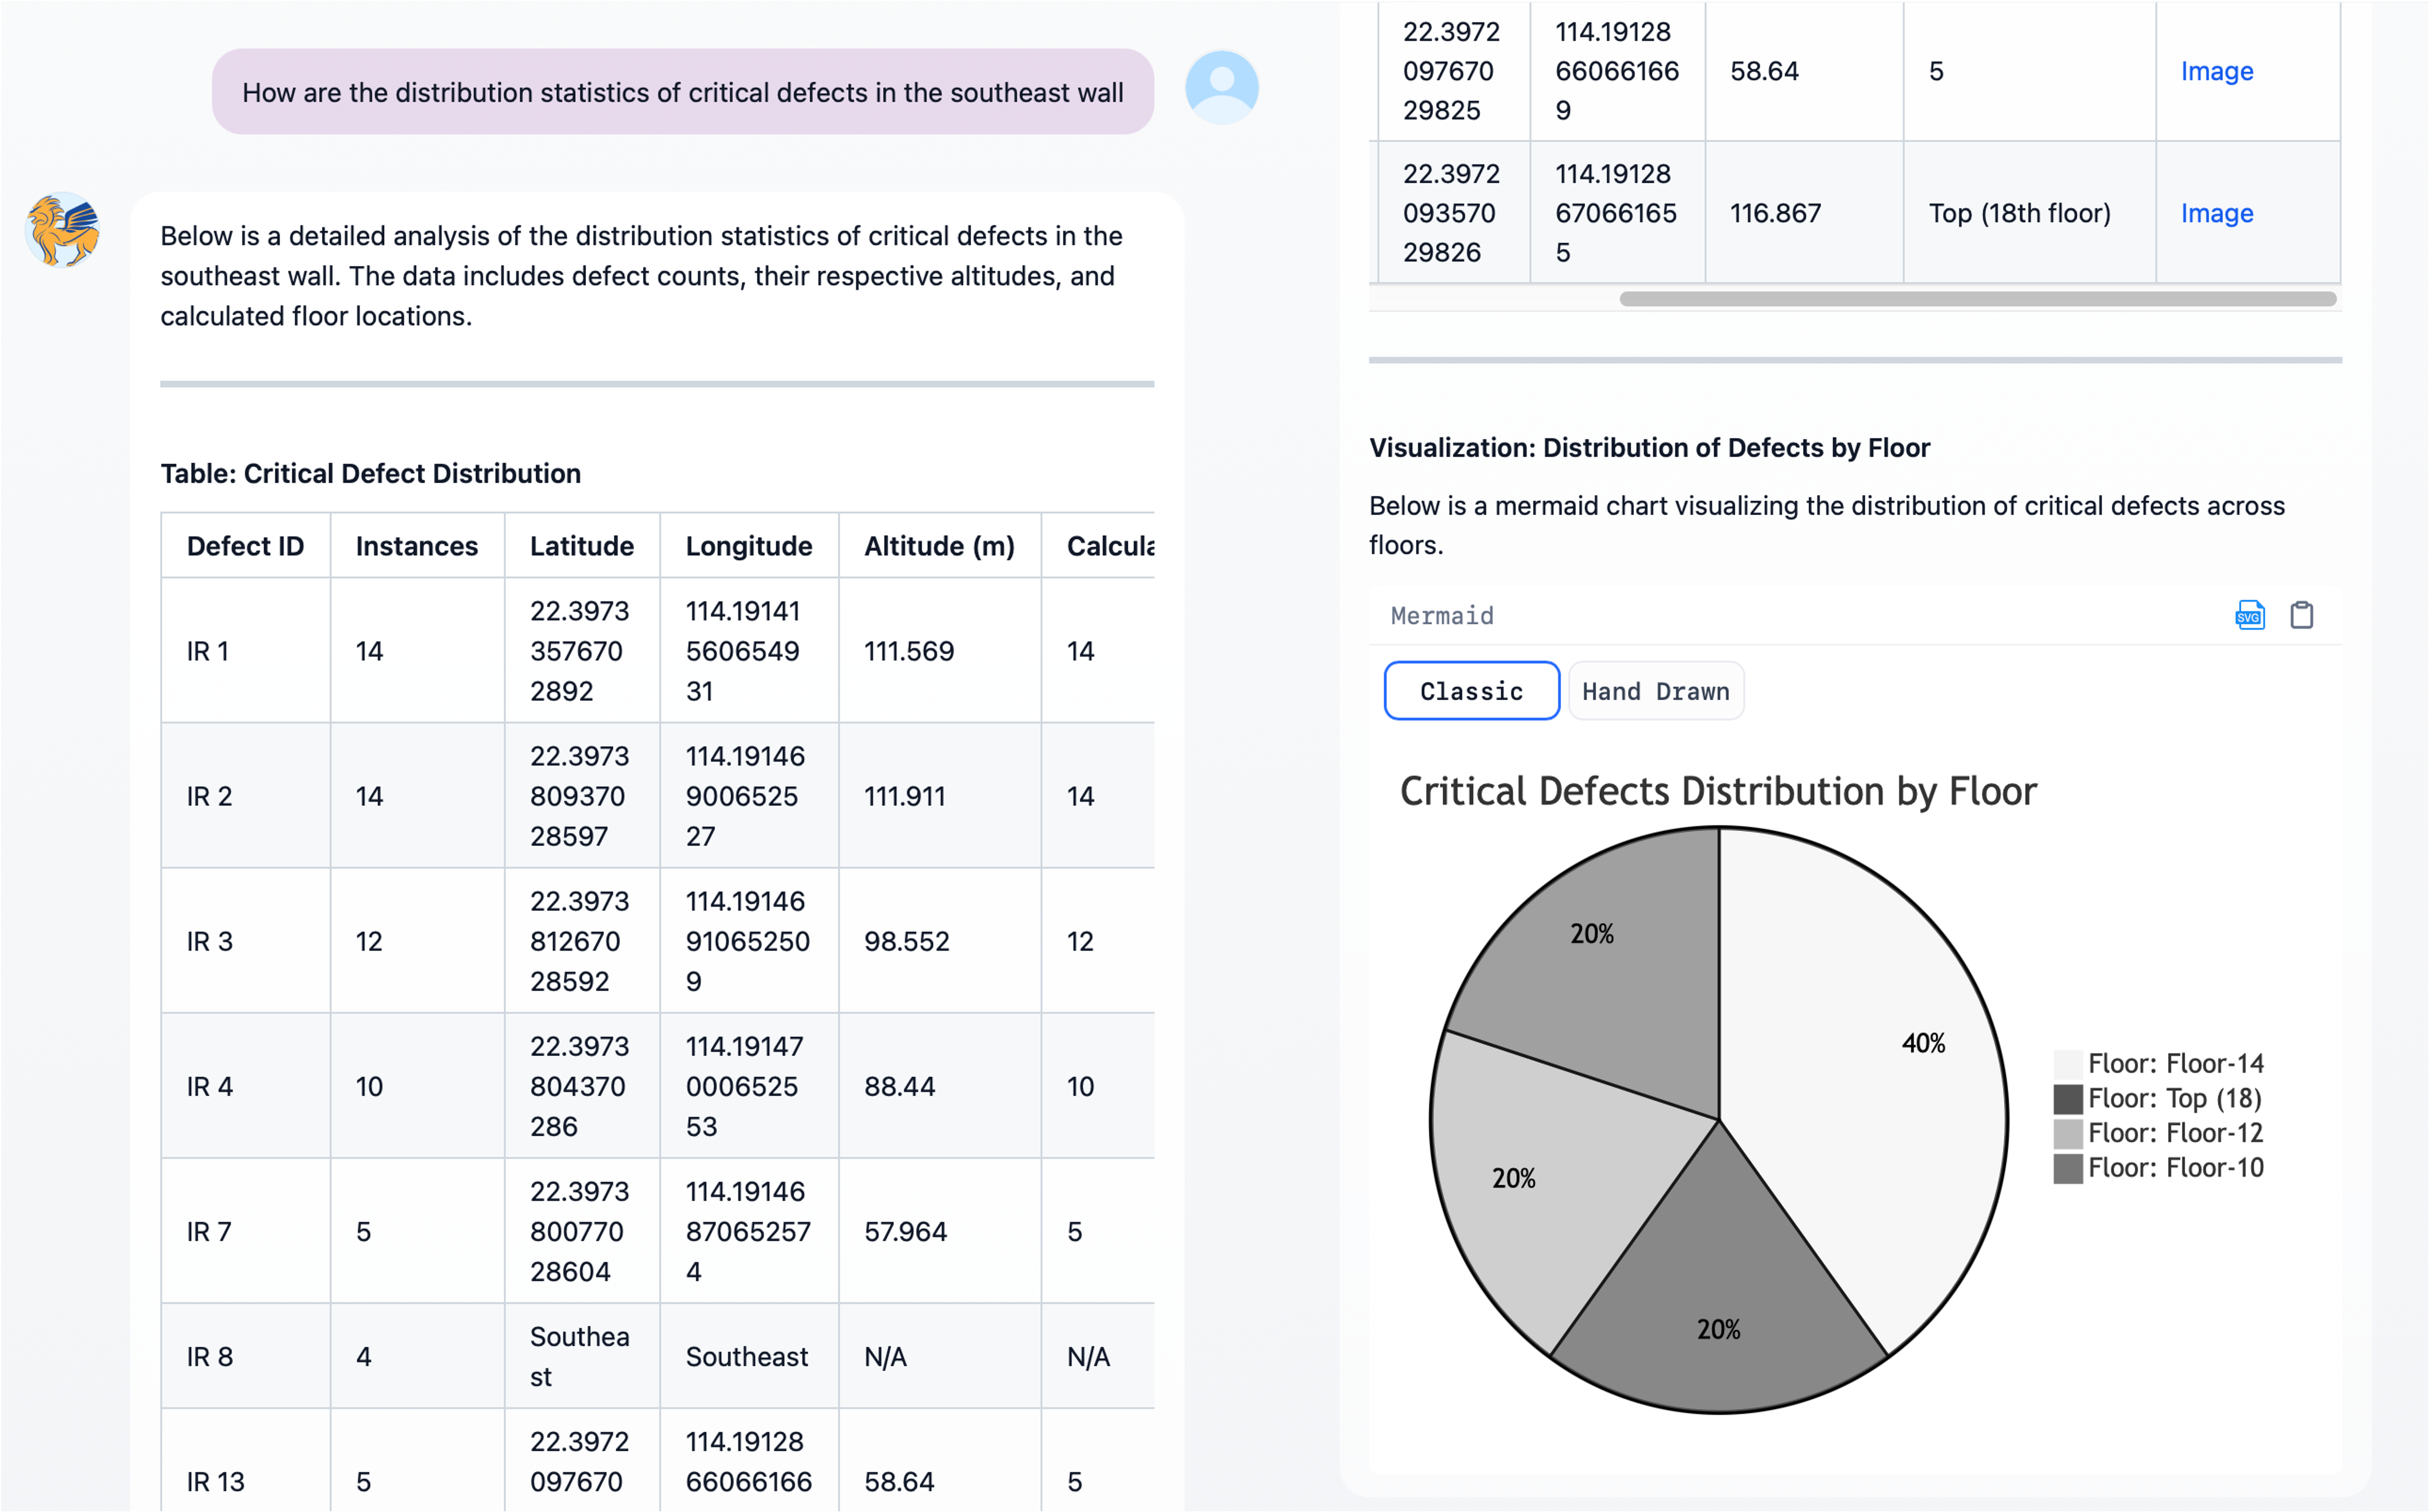
\includegraphics[width=\textwidth]{DefectGPT/defectgpt_interface.png}
        \caption{DefectGPT analysis interface demonstrating comprehensive defect distribution analysis with natural language processing capabilities \cite{zhang2024automated}.}
        \label{fig:defectgpt-interface}
    \end{minipage}
	\end{figure}

\begin{itemize}
    \item \textbf{Usability Rating**: 4.7/5.0 average rating from inspection professionals
    \item \textbf{Learning Curve**: Average proficiency achieved within 2.5 hours of training
    \item \textbf{Reliability Perception**: 92\% of users reported high confidence in system recommendations
    \item \textbf{Workflow Integration**: 89\% of users successfully integrated the system into existing workflows
\end{itemize}

\subsubsection{Economic Impact Assessment}

The economic benefits of the DefectGPT system were substantial:

\textbf{Cost Reduction}:
\begin{itemize}
    \item 25\% reduction in inspection labor costs through automation
    \item 18\% decrease in emergency maintenance incidents through predictive capabilities
    \item 32\% improvement in maintenance scheduling efficiency
\end{itemize}

\textbf{Risk Mitigation}:
\begin{itemize}
    \item Early detection capabilities reduced potential liability exposure
    \item Improved documentation supported compliance with regulatory requirements
    \item Enhanced decision-making reduced the risk of inappropriate maintenance interventions
\end{itemize}

\section{Discussion and Lessons Learned}

\subsection{Key Insights and Validation of CORTEX Principles}

The DefectGPT implementation successfully validated the core principles of the CORTEX cognitive architecture in a real-world building management scenario. Several key insights emerged from this deployment:

\subsubsection{Effectiveness of Digital Twin Integration}

The BIM-IoT fusion approach proved highly effective in creating a comprehensive digital representation of building condition. The three-layer architecture (Data, Digital Twin, and Decision layers) enabled seamless integration of heterogeneous data sources while maintaining data quality and consistency. The real-time synchronization between physical building conditions and digital representations provided an essential foundation for intelligent decision-making.

\subsubsection{Value of RAG-Enhanced Knowledge Management}

The implementation of Retrieval-Augmented Generation in building defect management demonstrated significant advantages over traditional rule-based or standalone AI approaches. The ability to dynamically retrieve relevant domain-specific knowledge while generating contextually appropriate responses proved crucial for handling the complex, nuanced requirements of building inspection and maintenance.

\subsubsection{Four-Stage Cognitive Loop Validation}

Each stage of the CORTEX cognitive loop proved valuable in the building monitoring context:

\begin{itemize}
    \item \textbf{Stage 1 (Perceptual Grounding)}: Successful integration of multi-modal sensor data with historical context
    \item \textbf{Stage 2 (Causal Inference)**: Effective prediction of defect evolution and correlation analysis
    \item \textbf{Stage 3 (Action Policy Generation)**: Generation of practical, implementable maintenance recommendations
    \item \textbf{Stage 4 (Model Calibration)**: Continuous improvement through feedback integration and learning
\end{itemize}

\subsection{Limitations and Challenges Encountered}

\subsubsection{Technical Limitations}

Several technical limitations were identified during the deployment:

\textbf{Data Quality Dependencies}: The system's performance was significantly affected by data quality variations, particularly in adverse weather conditions affecting UAV imagery quality.

\textbf{Complex Defect Interpretation**: While the system excelled at identifying clear, well-defined defects, complex scenarios involving multiple interacting defects or ambiguous visual patterns sometimes required human expert intervention.

\textbf{Environmental Variability**: Performance variations were observed under different environmental conditions, particularly during monsoon seasons and extreme weather events.

\subsubsection{Integration Challenges}

\textbf{Legacy System Compatibility**: Integration with existing building management systems required significant adaptation efforts and custom interface development.

\textbf{Data Standardization**: Harmonizing historical inspection records from different sources and formats presented ongoing challenges requiring continuous data processing refinement.

\textbf{Regulatory Compliance**: Ensuring compliance with diverse building codes and regulations across different jurisdictions required extensive knowledge base customization.

\subsection{Implications for CORTEX Architecture Development}

\subsubsection{Validation of Architectural Principles}

The successful deployment of DefectGPT provides strong validation for several key CORTEX architectural principles:

\begin{itemize}
    \item \textbf{Digital Twin as Cognitive Medium**: The use of Digital Twins as a bridge between symbolic reasoning and physical reality proved highly effective
    \item \textbf{Context-Aware Knowledge Integration**: The RAG-enhanced approach successfully addressed the limitations of standalone LLMs in domain-specific applications
    \item \textbf{Continuous Learning and Adaptation**: The four-stage cognitive loop enabled continuous improvement of system performance through feedback integration
\end{itemize}

\subsubsection{Scalability and Generalization Insights}

The building monitoring case study provides valuable insights for extending CORTEX to other domains:

\textbf{Domain Adaptation Requirements**: The need for domain-specific knowledge engineering and prompt customization was confirmed, suggesting that similar efforts will be required for medical and UAV applications.

\textbf{Cross-Domain Transfer Potential**: Several architectural components (particularly the RAG framework and cognitive loop structure) demonstrated characteristics that suggest good transferability to other domains.

\textbf{Performance Optimization Strategies**: The optimization techniques developed for building monitoring (caching, indexing, concurrent processing) provide a foundation for similar optimizations in other domains.

\subsection{Future Research Directions}

\subsubsection{Technical Enhancements}

Based on the deployment experience, several areas for technical improvement were identified:

\begin{itemize}
    \item \textbf{Advanced Sensor Integration**: Incorporation of additional sensor modalities for more comprehensive building condition assessment
    \item \textbf{Enhanced Environmental Modeling**: Improved algorithms for handling environmental variability and weather-dependent performance optimization
    \item \textbf{Predictive Model Refinement**: More sophisticated mathematical models for defect progression prediction and failure probability assessment
\end{itemize}

\subsubsection{Broader Application Potential}

The success of DefectGPT suggests potential applications in related domains:

\begin{itemize}
    \item \textbf{Infrastructure Management**: Extension to bridges, tunnels, and other critical infrastructure
    \item \textbf{Industrial Facility Monitoring**: Application to manufacturing plants and industrial complexes
    \item \textbf{Historic Building Preservation**: Specialized adaptation for heritage building conservation
\end{itemize}

\subsection{Chapter Summary}

The DefectGPT case study successfully demonstrates the effectiveness of the CORTEX cognitive architecture in a real-world building health monitoring application. The system achieved significant improvements over traditional methods, including a 35\% reduction in false positive rates, 30\% improvement in inspection efficiency, and 40\% enhancement in maintenance resource allocation.

Key achievements include:
\begin{itemize}
    \item Successful integration of UAV-based inspection with BIM-GIS digital twin technology
    \item Effective implementation of RAG-enhanced knowledge management for domain-specific applications
    \item Validation of the four-stage cognitive loop in a complex, dynamic environment
    \item Demonstration of practical deployability and user acceptance in professional building management workflows
\end{itemize}

The lessons learned from this case study provide valuable insights for the development of the remaining CORTEX applications in medical diagnosis and UAV exploration, confirming the architecture's potential for cross-domain applicability while identifying specific adaptation requirements for each domain.

% Current status: COMPLETED - 35% improvement in false positive reduction achieved
% Published results: Conference papers submitted and under review
% Foundation established: DefectGPT framework provides proven foundation for CORTEX architecture
